\section[Experimental Results]{Experimental Results and Comments}

\subsection[Experimental Data]{Tables of Experimental Data}
The following tables present the performance metrics (Running Time and Number of Comparisons) for five string matching algorithms evaluated under two different scenarios. 

\vspace{0.3cm}
\noindent\textit{Note: The number of comparisons for the Aho-Corasick algorithm is recorded as 0 across all test cases. This is due to its underlying architecture; rather than performing traditional character-by-character comparisons, it traverses a pre-constructed finite state automaton (Trie with failure links), making traditional comparison tracking inapplicable.}
\vspace{0.3cm}

\subsubsection*{Scenario 1: Varying Grid Size with Fixed Number of Keywords (5)}

% Scenario 1: Running Time Table
\begin{table}[H]
    \centering
    \resizebox{\textwidth}{!}{
    \begin{tabular}{|c|c|r|r|r|r|r|}
        \hline
        \textbf{Grid Size} & \textbf{Keywords} & \textbf{Brute Force} & \textbf{Rabin-Karp} & \textbf{KMP} & \textbf{Boyer-Moore} & \textbf{Aho-Corasick} \\ \hline
        $10 \times 10$ & 5 & 0.0739 ms & 0.0569 ms & 0.1547 ms & 0.1110 ms & 0.1718 ms \\ \hline
        $50 \times 50$ & 5 & 1.4625 ms & 0.3992 ms & 0.7692 ms & 0.4074 ms & 0.9691 ms \\ \hline
        $100 \times 100$ & 5 & 10.6593 ms & 0.6735 ms & 5.0648 ms & 0.6937 ms & 1.5499 ms \\ \hline
        $500 \times 500$ & 5 & 1167.3600 ms & 13.9877 ms & 17.7575 ms & 15.6578 ms & 35.1272 ms \\ \hline
    \end{tabular}
    }
    \caption{Running time measurements for Scenario 1}
\end{table}

% Scenario 1: Comparisons Table
\begin{table}[H]
    \centering
    \resizebox{\textwidth}{!}{
    \begin{tabular}{|c|c|r|r|r|r|r|}
        \hline
        \textbf{Grid Size} & \textbf{Keywords} & \textbf{Brute Force} & \textbf{Rabin-Karp} & \textbf{KMP} & \textbf{Boyer-Moore} & \textbf{Aho-Corasick} \\ \hline
        $10 \times 10$ & 5 & 2,520 & 18 & 3,172 & 236 & 0 \\ \hline
        $50 \times 50$ & 5 & 231,400 & 78 & 78,740 & 1,767 & 0 \\ \hline
        $100 \times 100$ & 5 & 1,836,800 & 986 & 282,803 & 22,880 & 0 \\ \hline
        $500 \times 500$ & 5 & 216,796,000 & 1,448 & 6,669,643 & 124,220 & 0 \\ \hline
    \end{tabular}
    }
    \caption{Number of comparisons for Scenario 1}
\end{table}

\vspace{0.5cm}
\subsubsection*{Scenario 2: Fixed Grid Size ($100 \times 100$) with Varying Number of Keywords}

% Scenario 2: Running Time Table
\begin{table}[H]
    \centering
    \resizebox{\textwidth}{!}{
    \begin{tabular}{|c|c|r|r|r|r|r|}
        \hline
        \textbf{Grid Size} & \textbf{Keywords} & \textbf{Brute Force} & \textbf{Rabin-Karp} & \textbf{KMP} & \textbf{Boyer-Moore} & \textbf{Aho-Corasick} \\ \hline
        $100 \times 100$ & 1 & 1.8014 ms & 0.1474 ms & 0.2855 ms & 0.1188 ms & 1.6196 ms \\ \hline
        $100 \times 100$ & 10 & 20.1295 ms & 1.1338 ms & 2.0147 ms & 1.1114 ms & 2.0038 ms \\ \hline
        $100 \times 100$ & 50 & 99.2332 ms & 5.4070 ms & 9.4388 ms & 5.1438 ms & 3.5454 ms \\ \hline
        $100 \times 100$ & 100 & 195.2980 ms & 11.0356 ms & 49.1021 ms & 10.8136 ms & 4.8826 ms \\ \hline
    \end{tabular}
    }
    \caption{Running time measurements for Scenario 2}
\end{table}

% Scenario 2: Comparisons Table
\begin{table}[H]
    \centering
    \resizebox{\textwidth}{!}{
    \begin{tabular}{|c|c|r|r|r|r|r|}
        \hline
        \textbf{Grid Size} & \textbf{Keywords} & \textbf{Brute Force} & \textbf{Rabin-Karp} & \textbf{KMP} & \textbf{Boyer-Moore} & \textbf{Aho-Corasick} \\ \hline
        $100 \times 100$ & 1 & 228,800 & 104 & 46,207 & 1,986 & 0 \\ \hline
        $100 \times 100$ & 10 & 3,663,600 & 451 & 643,058 & 7,001 & 0 \\ \hline
        $100 \times 100$ & 50 & 16,450,800 & 731 & 3,155,398 & 54,562 & 0 \\ \hline
        $100 \times 100$ & 100 & 34,552,800 & 3,529 & 6,225,769 & 174,645 & 0 \\ \hline
    \end{tabular}
    }
    \caption{Number of comparisons for Scenario 2}
\end{table}

\newpage
\subsection[Evaluation]{Performance Evaluation and Comments}

Based on the experimental data presented above, the following observations and justifications address the core performance behaviors of the implemented algorithms.

\begin{itemize}
    \item \textbf{Correlation with Big-O Complexity:}\\
    The growth rates observed in the experimental data heavily align with the theoretical Big-O complexities of the algorithms. 
    \begin{itemize}
        \item \textbf{Brute Force:} In Scenario 1, as the grid size increases from $10 \times 10$ to $500 \times 500$, the running time explodes from $0.0739$ ms to $1167.36$ ms, and comparisons reach over 216 million. This perfectly illustrates its $O(N \cdot M)$ worst-case complexity, where $N$ is the text size and $M$ is the pattern size. It must redundantly check every possible starting position.
        \item \textbf{Aho-Corasick:} In Scenario 2, as the number of keywords increases from 1 to 100, Brute Force and KMP show linear growth in execution time. However, Aho-Corasick exhibits an incredibly flat growth curve (increasing only from $1.6196$ ms to $4.8826$ ms). This matches its theoretical complexity of $O(N + M + Z)$ (where $Z$ is the number of matches). Because it builds an automaton, the search time relies primarily on the length of the text, remaining largely independent of the number of patterns being searched simultaneously.
    \end{itemize}

    \vspace{0.2cm}
    \item \textbf{Best Performers on Large Datasets vs. Small Datasets:}\\
    The "best" algorithm depends entirely on the nature of the dataset.
    \begin{itemize}
        \item For a \textbf{large search space (Grid $500 \times 500$) with few keywords}, \textbf{Rabin-Karp} ($13.9877$ ms) and \textbf{Boyer-Moore} ($15.6578$ ms) performed the best. Boyer-Moore's efficiency is evident in its low comparison count ($124,220$), as its bad-character heuristic allows it to skip large sections of the text.
        \item For a \textbf{large dictionary of keywords (100 keywords)}, \textbf{Aho-Corasick} is the absolute best performer ($4.8826$ ms), outperforming the next fastest (Boyer-Moore at $10.8136$ ms) by more than double the speed.
    \end{itemize}
    
    \textbf{The Brute Force Exception:} There is a clear case where Brute Force was faster than the optimized approaches. In \textbf{Scenario 1, at the smallest grid size ($10 \times 10$) with 5 keywords}, Brute Force ($0.0739$ ms) outperformed KMP ($0.1547$ ms), Boyer-Moore ($0.1110$ ms), and Aho-Corasick ($0.1718$ ms).

    \vspace{0.2cm}
    \item \textbf{Justification of Results:}\\
    The phenomenon where Brute Force beats advanced algorithms on very small datasets is due to \textbf{preprocessing overhead}. Algorithms like KMP, Boyer-Moore, and Aho-Corasick require initial time to construct LPS arrays, shift tables, or complex automata before the search even begins. On a tiny $10 \times 10$ grid, the time taken to build these data structures exceeds the time it takes for Brute Force to simply execute nested loops to check the few available characters.
    
    Conversely, on large datasets, this preprocessing overhead pays off immensely. Rabin-Karp shows an astonishingly low number of comparisons (e.g., only 1,448 comparisons for a $500 \times 500$ grid) because it compares integer hash values rather than full strings, only resorting to character comparisons when a hash collision occurs. Meanwhile, Aho-Corasick dominates the multiple-keyword scenario because its automaton processes the grid exactly once, finding all 100 keywords simultaneously, whereas all other algorithms must iterate through the grid repeatedly for every single keyword.
\end{itemize}

\newpage
\newpage
\subsection[Graphs]{Tables and Graphs}

\begin{figure}[H]
    \centering
    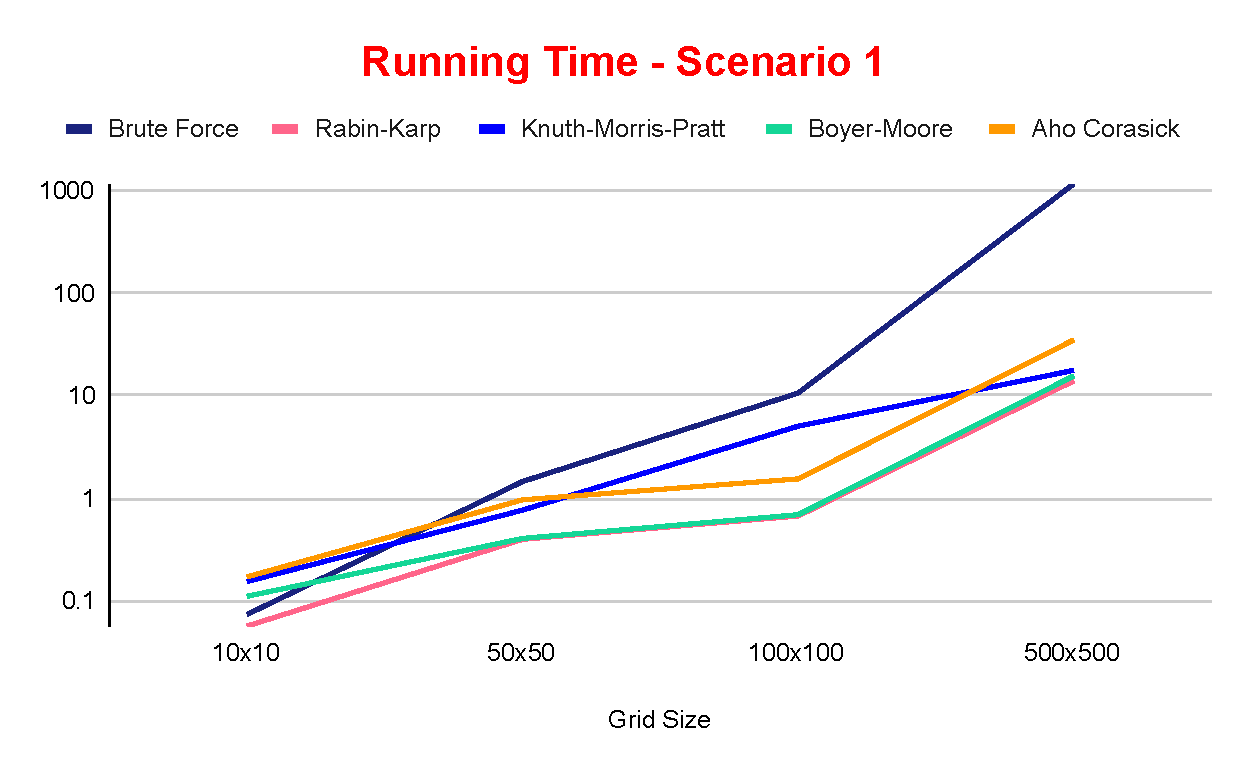
\includegraphics[width=\textwidth]{data/Graph/time1.pdf}
\end{figure}

\vspace{1cm}

\begin{figure}[H]
    \centering
    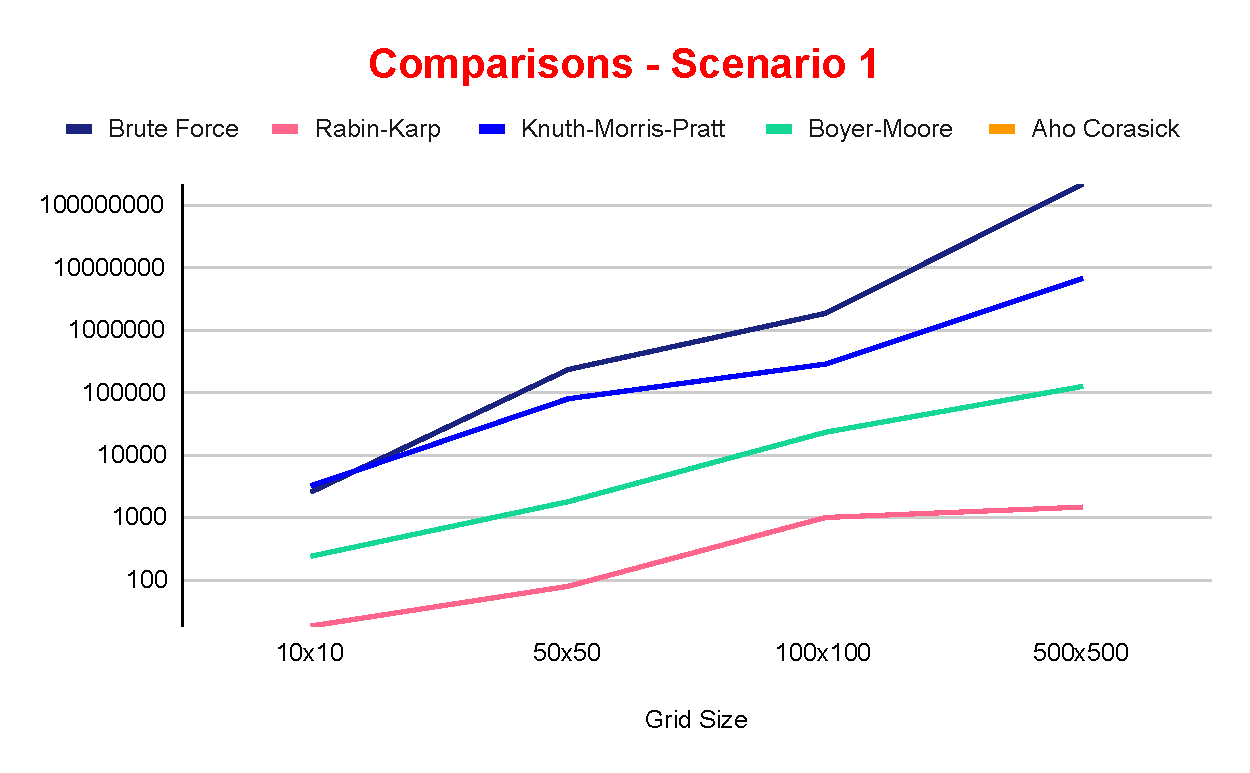
\includegraphics[width=\textwidth]{data/Graph/comp1.pdf}
\end{figure}

\newpage

\begin{figure}[H]
    \centering
    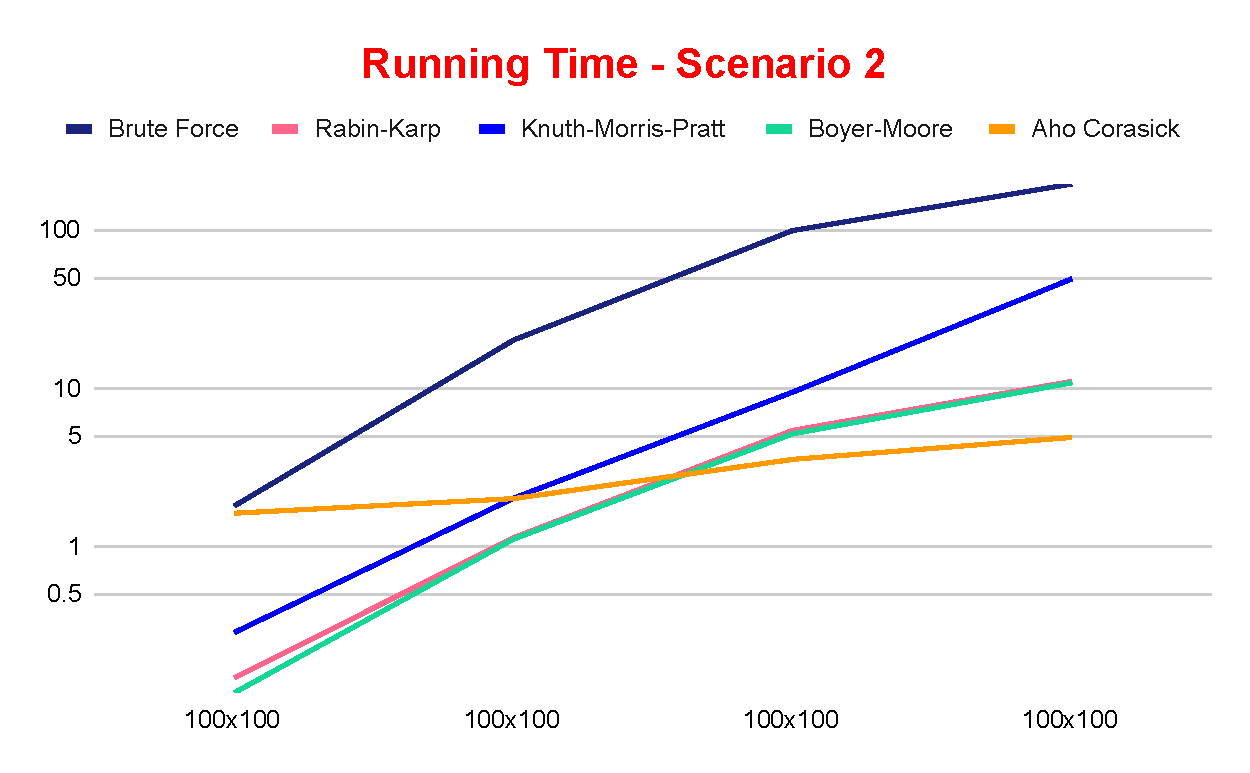
\includegraphics[width=\textwidth]{data/Graph/time2.pdf}
\end{figure}

\vspace{1cm}

\begin{figure}[H]
    \centering
    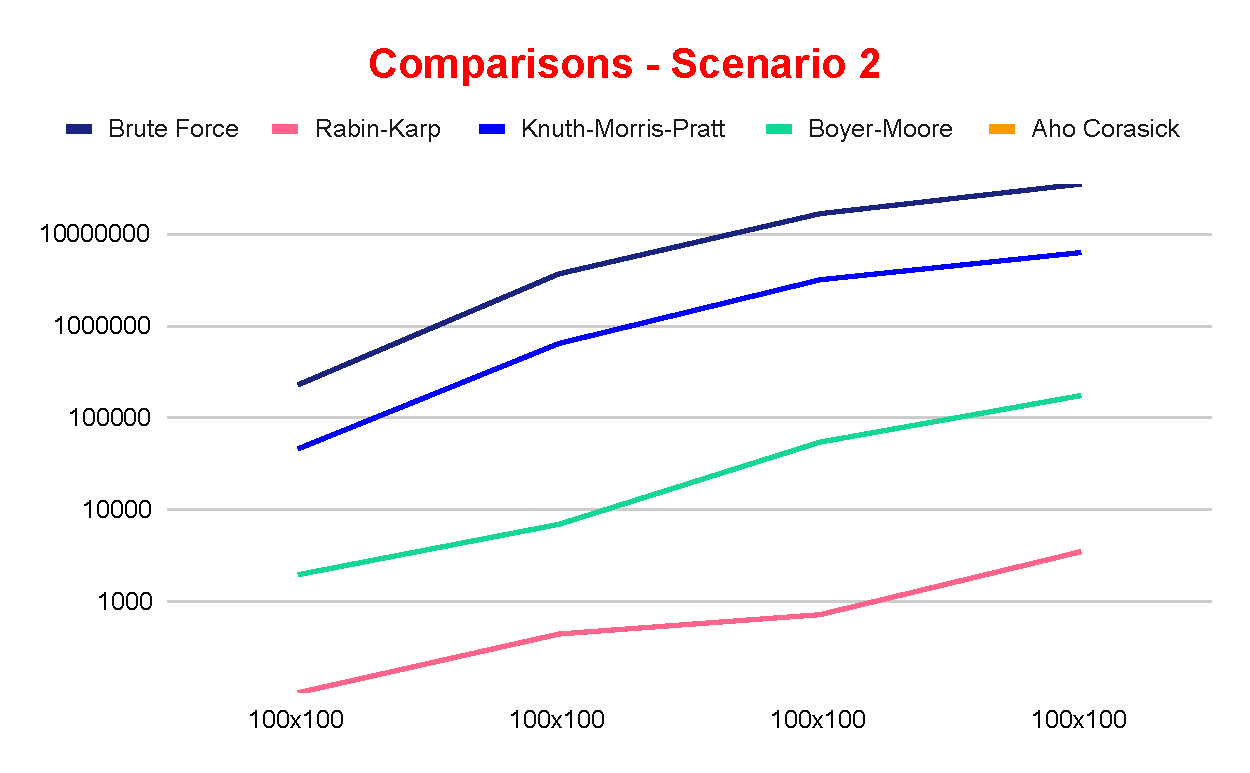
\includegraphics[width=\textwidth]{data/Graph/comp2.pdf}
\end{figure}